\chapter{Simulations with \software}

	\software was programmed to simulate spherical nanocrystals and to visualize the results of the simulations.
	Though we focused on spherical structures, the code is hold abstract and slim to make extending to other
	structures, such as nanowires, fairly easy.
	The main aim of \software is to offer \omen users a toolbox, which includes the following 3 main tasks:
	\begin{enumerate}
		\itemsep 0pt
		\item Automatization of the \omen simulation process \\
					When it comes to simulating quantum dots with different parameters users do not want to spend a lot
					of time on writing command files for OMEN by themselves and start each OMEN task via the shell, but 
					rather enter the main parameters into a \gls{GUI} and let \software do the rest (see section \ref{sec:RunSim}).
					This makes overnight simulations for large parameter sets possible.
		\item Overview of all simulations done in the past	\\
					All information respectively parameters of past simulations can be displayed in a \gls{GUI}. Exporting selected
					simulations and visualizing them is possible as well (see section \ref{sec:guiDB})
		\item Visualization of simulation data	\\
					All different kinds of plots are available within the toolbox, such as visualizing band gaps, wave functions or
					quantum dot structures (see section \ref{sec:Visualization}).
	\end{enumerate}

	\section{Installing the Software}
		*********************** \\
		****** TO DO !!! ****** \\
		*********************** \\
	
	\section{Using \software}
		\subsection{Running a simulation} \label{sec:RunSim}
			Type gui\_simulate \index{gui\_simulate} in the \matlab command window and hit enter. The window as in figure \ref{fig:gui_simulate} will open.
			\begin{figure}[htbp]
				\centering
				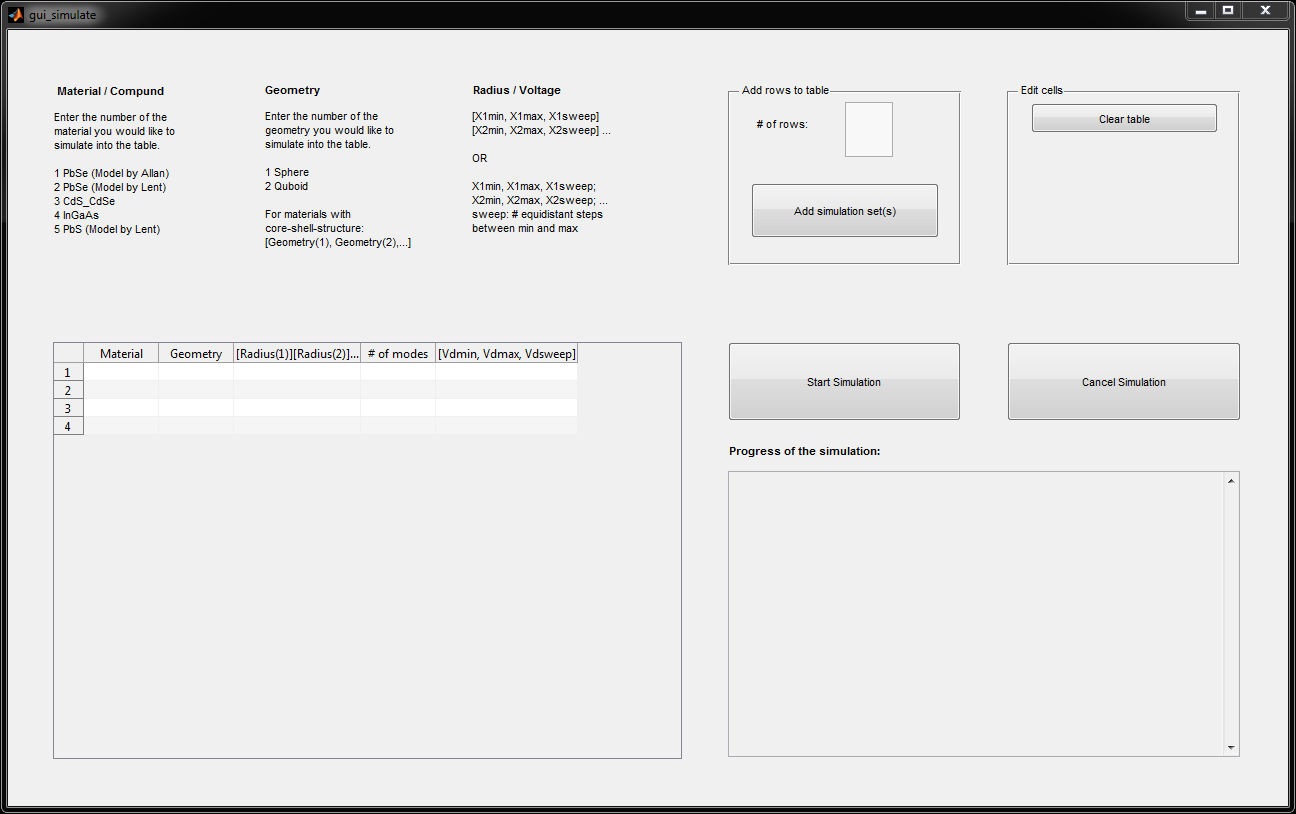
\includegraphics[width=0.6\textwidth]{Fig/Scrn_gui_simulate.png}
				\caption{The gui\_simualte window}
				\label{fig:gui_simulate}
			\end{figure}
			A simulation set is defined as one row of the table, i.e one material with all kinds of sweeps. You can add more simulation sets
			by using the {\it Add rows to the table} panel.
			It is possible to copy and paste single cells of the table using the appropriate short cuts of your \matlab default keyboard setup
			(\verb|CTRL+C & CTRL+V| Windows setting, \verb|ALT+W & CTRL+Y| Emacs setting).
			The columns are filled as follows:
			\begin{enumerate}
				\item Material		\\
							Enter the number for the material you would like to simulate, according to the {\it Material / Compound} list.
				\item Geometry		\\
							Enter the number of the geometry given in the {\it Geometry} list. Very important in the case of materials with
							shells is, that you have to enter the geometry type of the core and the shell. The geometry types are separated	
							with a comma.
							\begin{EXAMPLE}
								For a spherical CdS-CdSe quantum dot the cell would look like this: 1, 1
							\end{EXAMPLE}
				\item Radius			\\
							The radius has to be entered in a specific way. The syntax is: \\
							\verb|[Rmin(1), Rmax(1), Rsweep(1)][Rmin(2), Rmax(2), Rsweep(2)]...| \\
							\newline
							\begin{tabular}{@{}ll}
								\verb|Rmin(i)|		& smallest radius of the i\textsuperscript{th} material to be simulated				\\
								\verb|Rmax(i)|		& largest radius of the i\textsuperscript{th} material to be simulated				\\
								\verb|Rsweep(i)|	& number of equidistant points between \verb|Rmin(i)| \& \verb|Rmax(i)|		\\
							\end{tabular}
							
							\begin{EXAMPLE}
								Simulation a single spherical PbS quantum dot with radius 3.5 nm you would enter: [3.5,3.5,1]
							\end{EXAMPLE}
							
							\begin{EXAMPLE}
								For a spherical CdS-CdSe quantum dot the cell would look like this: [1,4,4][5,6,2]
								Looking at the radius parameters, \software will do all the permutations and generate therefore 8 quantum dots: \\
								\newline
								\begin{tabular}{@{}lcccccccc}
									Quantum dot					&	1	&	2	&	3	&	4 &	5	&	6	& 7	&	8	\\
									Core radius	in nm		&	1	& 1 & 2 & 2 & 3	& 3 & 4 & 4	\\
									Shell radius in nm	& 5	& 6 & 5 & 6 & 5 & 6 & 5 & 6	\\
								\end{tabular}
							\end{EXAMPLE}
				\item \# of modes	\\
							Enter a number of modes you would like to calculate.
				\item Voltage			\\
							The Voltage sweep is entered in the same way as the radius. You find more information under the following remark.
			\end{enumerate}
			
			\begin{REMARK}[Vectors \& Matrices] \index{Vector}
				As the \matlab \gls{GUI}s do not accept vectors or matrices as it is known from the command window, the parameters
				have to be entered as a string and are converted to matrices later on.
				
				There are different ways how to enter the parameters. Use the one, that is the most clear for you.
				\begin{verbatim}
               a,b,c,...,d                 or
              [a,b,c,...,d]                becomes a double vector

              V = [ a b c ... d]


              [a,b,c][d,e,f]...[g,h,j]     or
               a,b,c; d,e,f;...;g,h,j      or
              [a,b,c; d,e,f;...;g,h,j]     becomes a double matrix

              M = [ a b c
                    d e f
                    . . .
                    g h j ]

              where a,b,...,j are doubles as strings.
   			\end{verbatim}
   			These input styles can be applied to column {\it Geometry}, {\it Radius} and {\it Voltage}.	\\
   			You can use as many spaces as you want in between. The first and the last brace are not necessary if only a vector is entered or if
   			rows are separated by semicolons.
			\end{REMARK}
			
			After entering all the necessary parameters proceed by clicking \verb|Start Simulation|. The {\it Progress of the simulation} panel will
			keep you informed about the warnings, wrong entered parameters and the current status of the simulation.



		\subsection{Display simulation information} \label{sec:guiDB}
			There are two ways of displaying simulation information, either you can see the whole database \index{Database} (all simulations
			that are stored in the Simulations folder) or only specific data, for example only PbS simulation data.
			
			\begin{REMARK}
				\software uses objects (called {\it qdotObj}) to store all important data of simulations such as the simulation parameters, date of simulation etc.
				(futher information section \ref{sec:SoftwareStructure}). All operations are done using these objects. If you would like to display only
				certain simulation data, you would need an {\it qdotObj} array. How to create such an array please read section \ref{sec:addTools}.
			\end{REMARK}
			
			Displaying the whole database can be done by typing \verb|gui_db| \index{gui\_db} into the \matlab command window. A window as in figure \ref{fig:gui_database} will appear
			showing all parameters and technical information of each simulation. Please note, that according to the size of the database, it might take some seconds
			to load all data.
			If you only want to display a set of simulation data, you can also call \verb|gui_db(qdotObj_ARRAY)|, where \verb|qdotObj_ARRAY| is an array of qdotQbj objects.
			
			\begin{figure}[htbp]
				\centering
				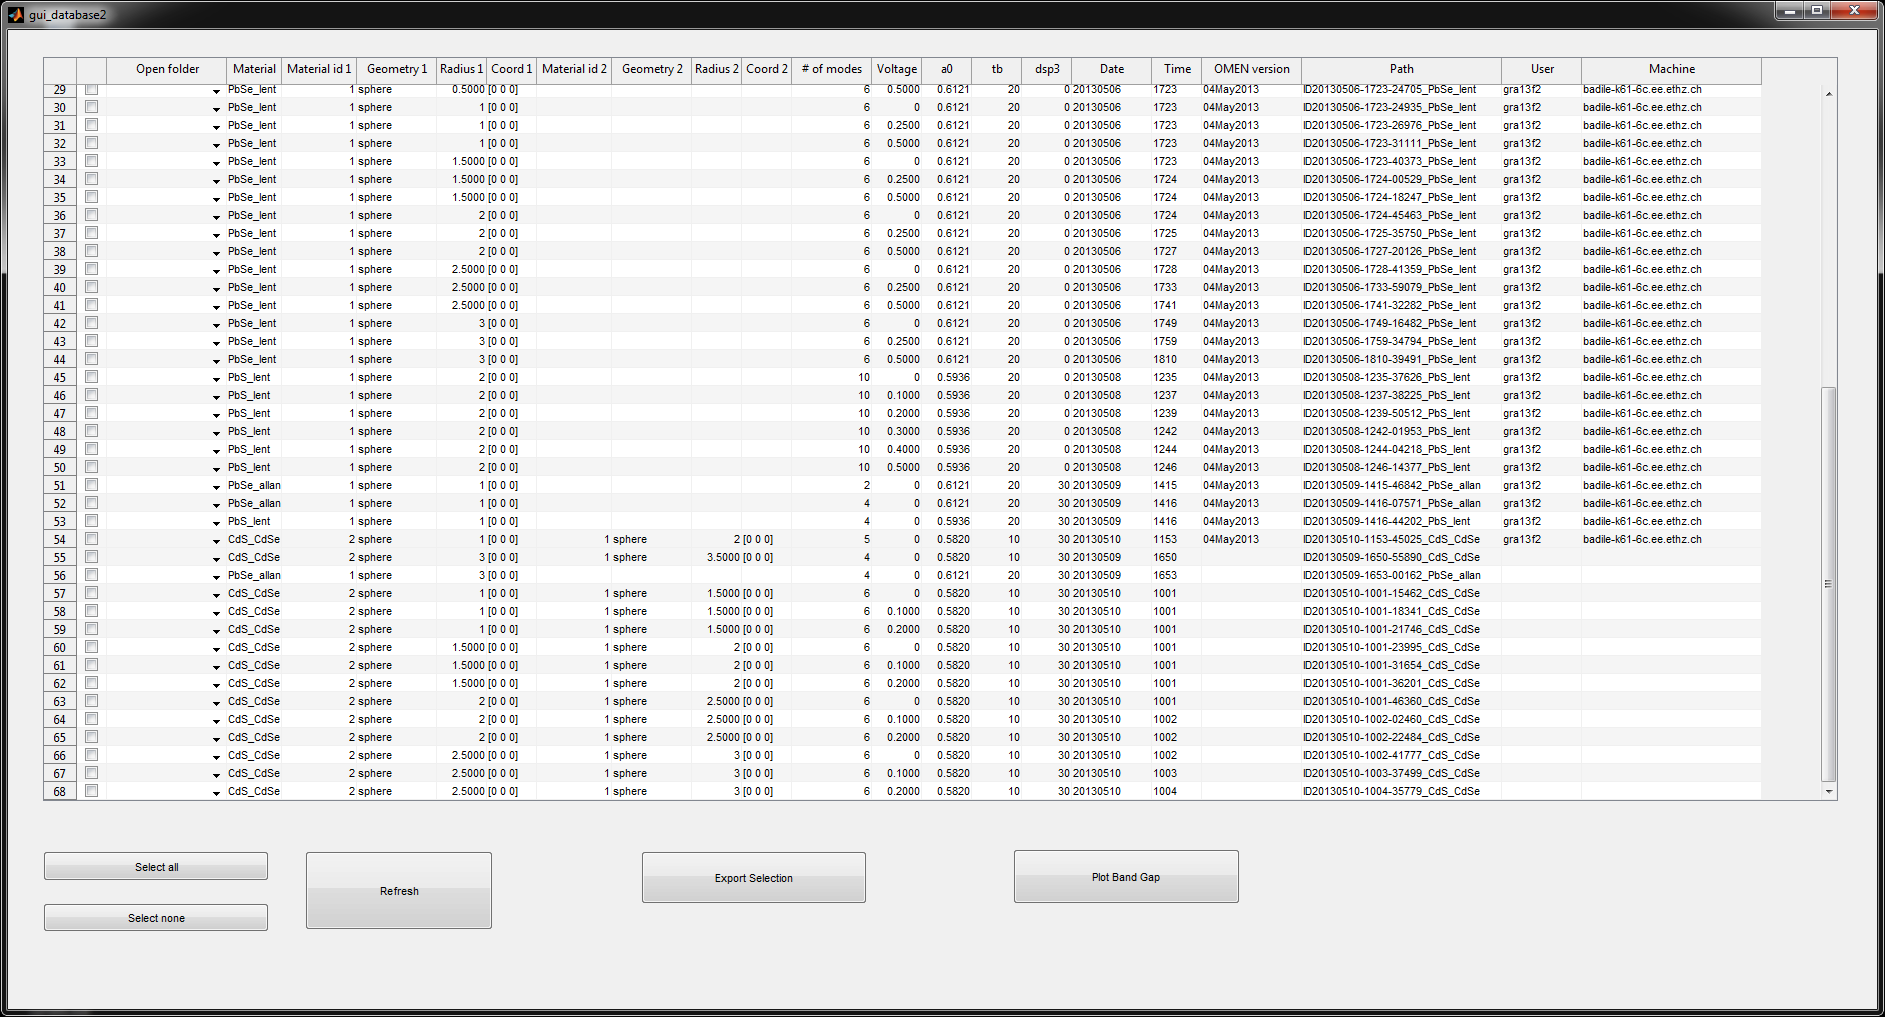
\includegraphics[width=\textwidth]{Fig/Scrn_gui_database.png}
				\caption{The gui\_database window}
				\label{fig:gui_database}
			\end{figure}
			
			Within the \gls{GUI} you can sort the simulations with the column header, select simulations and let plot them, open the directory of a simulation or 
			even export a selection, which is available as an qdotObj array in the main workspace entitled {\it ExportedDB}.


		\subsection{Visualization} \label{sec:Visualization}
			As explained in the previous section, simulation data can be visualized \index{Visualization} through the {\it gui\_database} window, but also manually.
			In this section the plotting \index{Plotting} functions are explained.
			
			\begin{lstlisting}
				plotBandGap(DB)
			\end{lstlisting}
		
		
		\subsection{Additional tools} \label{sec:addTools}
			
	
	\section{Maintaining \software}
		\subsection{General Structure} \label{sec:SoftwareStructure}
		
			\begin{figure}[htbp]
				\begin{minipage}[b]{0.59\textwidth}
				% Creates a directory structure figure
				\dirtree{%
				.1 /root.
					.2 MATLAB.
						.3 Classes.
						.3 Functions.
						.3 GUI.
						.3 System.
					.2 OMEN executable.
					.2 Simulations.
						.3 ID*.
						.3 \vdots.
						.3 log.
				}
				\caption{The \software structure by default}
				\label{dir:ToolboxTree}
			\end{minipage}
			\hfill
			\begin{minipage}[b]{0.39\textwidth}
			\dirtree{%
			.1 ID*.
				.2 CB\_E\_0\_0.dat.
				.2 CB\_V\_0\_0.dat.
				.2 H\_0.dat.
				.2 Layer\_Matrix.dat.
				.2 qdot\_cmd.
				.2 qdotObj.mat.
				.2 simlog\_{\it yyyymmdd\_hhmm\_ssfff}.
				.2 VB\_E\_0\_0.dat.
				.2 VB\_E\_0\_0.dat.
			}
			\caption{Structure of a simulation set}
			\label{dir:SimSetTree}
			\end{minipage}
			\end{figure}
			
			\begin{lstlisting}[frame=single]
				IDyyyymmdd-hhmm-ssfff_MATNAME
			\end{lstlisting}
				
			\begin{lstlisting}[frame=single]
			struct global config {
				config.root        = '';
				config.system      = '';
				config.log         = '';
				config.user        = '';
				config.machine     = '';
				config.OMEN        = '';
				config.simulations = '';
				config.vOMEN       = '';
				config.cancelSim   = '';
			}
			\end{lstlisting}
			
%	\subsection{Installing and setting up \software}
%		\subsection{\acl{GUI}}
%			\subsubsection{Starting a new Simulation}
%			
%			\subsubsection{}
%		
%		\subsection{OMEN Procedures}
%		
%		\subsection{Visualization}